Im folgenden sind einige Algorithmen aufgeführt, mit denen rechteckige Labyrinthe generiert werden können.
Zum schluss ist in Abschnitt~\ref{subsec:unsere-implementierung} unsere, auf den Vor\- und Nachteilen der aufgeführten Algorithmen basierte Entscheidung, der \qq{Randomised-Depth-First-Search} Algorithmus, weiter ausgeführt.
\subsection{Randomized-Depth-First-Search}\label{subsec:randomized-depth-first-search}
    \begin{figure}[ht!]
        \centering
        \includegraphics[width=\paperwidth/2]{../assets/img/Randomised-Depth-First-Search}
        \caption{Randomized-Depth-First-Search Ablauf}
        \label{fig:randomized-depth-first-search-flow}
    \end{figure}
    Gegeben ist ein Feld der Breite $w$ und Höhe $h$.
    Das Feld beinhaltet alle Punkte $p\in\{(x,y)\in\mathbb{N}^2, 0\leq x<w, 0\leq y<h\}$.
    Daraus wird zunächst ein beliebiger Startpunkt ausgewählt.
    Die benachbarten Punkte werden nach Punkten durchsucht, die noch keine Verbindungen haben.
    Der Startpunkt wird zufällig mit einem dieser Punkte verbunden.
    Anschließend wird der verbindungspunkt zum neuen Startpunkt.
    Hat der Startpunkt keine benachbarten Punkte ohne Verbindungen, so wird der vorherige Startpunkt überprüft.
    Dies wird wiederholt, bis es keinen Punkt mehr gibt, der keine Verbindung hat.
    Der Ablauf ist auch in Abbildung~\ref{fig:randomized-depth-first-search-flow} dargestellt.

\subsection{Unsere Implementierung}\label{subsec:unsere-implementierung}
    \begin{figure*}[ht!]
        \lstinputlisting[label={lst:randomised-depth-first-search-code}, caption={Randomized-Depth-First-Search Implementierung}, language=java]{../assets/code/recursive_randomised_depth_first_search.java}
    \end{figure*}
    Wir haben uns für den \qq{Randomised-Depth-First-Search} Algorithmus entschieden, da dieser in einer guten Laufzeit von $\Theta(n)$\footnote{Im worst-- sowie bestcase braucht der Algorithmus $n\cdot x+h$ Sekunden, wobei $n$ die Anzahl der Felder ist und $x,h\in\mathbb{R}^+$.} hat und subjektiv schöne Abzweigungen generiert.


    Zunächst haben wir eine rekursive Implementierung gewählt.
    Dies ist zwar bei der Beschreibung des Algorithmus intuitiver, wollen wir jedoch große Labyrinthe generieren, so kann es zu einer StackOverflowException kommen, weshalb auch noch eine iterative Implementierung geplant ist.


    Als Datenmodell dient uns ein ungerichteter Graph.
    Graphen sind eine ansammlung von Knoten, die über Kanten miteinander verbunden sind.
    (Siehe Abbildung~\ref{fig:what-is-a-graph})
    Knoten haben einen Wert und Kanten setzen diese in Relation.
    Ungerichtet heißt dabei, dass die Verbindung in beide richtungen gild.
    \begin{figure}[ht!]
        \centering
        \begin{tabular}{l c}
            Liste &
            \begin{minipage}{0.7\textwidth}
                \centering
                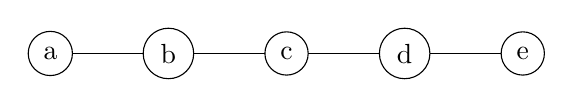
\begin{tikzpicture}[node distance={15mm}, main/.style = {draw, circle,outer sep=0pt}]
                    \node[main] (a) {a};
                    \node[main] (b) [right of=a] {b};
                    \node[main] (c) [right of=b] {c};
                    \node[main] (d) [right of=c] {d};
                    \node[main] (e) [right of=d] {e};

                    \draw (a) to (b);
                    \draw (b) to (c);
                    \draw (c) to (d);
                    \draw (d) to (e);

                    \title{Liste}
                \end{tikzpicture}
            \end{minipage}\\
            \vspace{15mm}\\
            Baum &
            \begin{minipage}{0.7\textwidth}
                \centering
                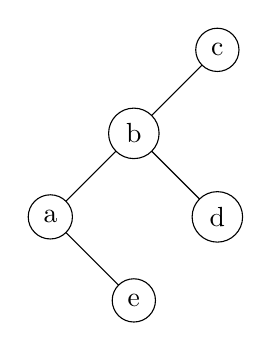
\begin{tikzpicture}[node distance={15mm}, main/.style = {draw, circle,outer sep=0pt}]
                    \node[main] (a) {a};
                    \node[main] (b) [above right of=a] {b};
                    \node[main] (c) [above right of=b] {c};
                    \node[main] (d) [below right of=b] {d};
                    \node[main] (e) [below right of=a] {e};

                    \draw (a) to (b);
                    \draw (b) to (c);
                    \draw (b) to (d);
                    \draw (a) to (e);


                    \title{Baum}
                \end{tikzpicture}
            \end{minipage}\\
            \vspace{15mm}\\
            Graph &
            \begin{minipage}{0.7\textwidth}
                \centering
                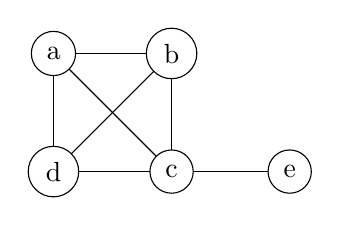
\begin{tikzpicture}[node distance={15mm}, main/.style = {draw, circle,outer sep=0pt}]
                    \node[main] (a) {a};
                    \node[main] (b) [right of=a] {b};
                    \node[main] (c) [below of=b] {c};
                    \node[main] (d) [left of=c] {d};
                    \node[main] (e) [right of=c] {e};

                    \draw (a) to (b);
                    \draw (b) to (c);
                    \draw (c) to (d);
                    \draw (d) to (a);
                    \draw (a) to (c);
                    \draw (b) to (d);
                    \draw (c) to (e);

                    \title{Graph}
                \end{tikzpicture}
            \end{minipage}
        \end{tabular}

        \caption{Was ist ein Graph?}
        \label{fig:what-is-a-graph}
    \end{figure}
    In unserem Fall ist der wert die Koordinate als Punkt $p\in\{(x,y)\in\mathbb{N}^2, 0\leq x<w, 0\leq y<h\}$.
    Da die Dimensionen bekannt sind, ist die Menge aller Punkte $P$ abzählbar (eine endliche Menge).
    Dies gestaltet die Implementierung einfach, da so nur die Kanten gespeichert werden müssen.


    Mit diesen Voraussetzungen fangen wir nun in Code~\ref{lst:randomised-depth-first-search-code} mit einem Startpunkt \lstinline{current} an und lassen uns solange alle anliegenden Knoten ohne Verbindung ausgeben, bis es keine mehr gibt.
    Mit einem zufälligen dieser Punkte aus \lstinline{adjacent} wird nun fortgefahren.
    Auf unserem Graphen verbinden wir die Knoten an den beiden Punkten.
    Danach wird die gegebene Methode rekursiv erneut aufgerufen, dieses mal mit dem ausgewählten Punkt.